\documentclass[11pt]{report}
%\usepackage{fancybox}
\usepackage{geometry}
\usepackage{amsmath}
\usepackage{txfonts}
\usepackage{layout}
\usepackage{setspace}
%\usepackage{mathptmx}
\geometry{a4paper, left=22mm, right=22mm, top=25mm, bottom=25mm}
\usepackage{wrapfig}
\usepackage[dvipdfm]{graphicx,hyperref}
\usepackage{mediabb}
\setstretch{1.3}
\title{\Huge\bf{Role of Noncollective Excitations in Low-Energy Heavy-Ion Fusion Reaction
and Quasi-Elastic Scattering}}
\author{\\\\\\\\\\\\\\\\\\\\\\\\\\\\{\it\Large Department of Physics, Faculty of Science, Tohoku University}\\\\
\Huge Shusaku Yusa}
\date{March, 2013}
\begin{document}


\chapter{Coupled-channels method}
In this chapter, a theoretical framework which
we employ in this thesis for the description of heavy-ion reactions, 
that is, the coupled-channels method is detailed.
After introducing the concept of barrier distribution for fusion and quasi-elastic
scattering, the effects of collective excitations on the barrier
distributions are presented.

\section{Coupled-channels equations}
The coupled-channels method describes the coupling of the relative motion
to the intrinsic degrees of freedom of the colliding nuclei, that is, the
excitations during the scattering process.
%The wave function in this method is represented as a superposition of various
%channel wave functions.
The coupled-channels method assumes the following Hamiltonian
\begin{eqnarray}
  H = -\frac{\hbar^2}{2\mu}\nabla^2 + V_0(r) + H_0(\xi) 
+ V_{\rm coup}(\bvec{r},\xi), 
\end{eqnarray}
where $\bvec{r}$ is the coordinate for the relative motion between the 
projectile and
the target nuclei, and $\mu$ is the reduced mass.  
$H_0(\xi)$ is the intrinsic Hamiltonian, and
$\xi$ represents the internal degrees of
freedom. 
$V_0(r)$ is the optical potential for the relative motion.
This includes an imaginary part to represent the loss of flux from the
considered model space. 
$V_{\rm coup}(\bvec{r},\xi)$ is the coupling Hamiltonian between 
the relative motion and the intrinsic degrees of freedom. 
We expand $V_{\rm coup}(\bvec{r},\xi)$ in terms of spherical harmonics as
\begin{eqnarray}
V_{\rm coup}(\bvec{r},\xi) = \sum_{\lambda >0}f_{\lambda}(r)
Y_{\lambda}(\hat{\bvec{r}})\cdot T_{\lambda}(\xi),
\label{eq3.2}
\end{eqnarray}
where, the dot represents a scalar product.
The monopole term ($\lambda = 0$) 
in the interaction is assumed to be contained in $V_{0}(r)$ and 
not included in $V_{\rm coup}$.
Although one can assume more general expansion
$\displaystyle
V_{\rm coup}(\bvec{r},\xi) = \sum_{\alpha}\sum_{\lambda >0}f_{\lambda}^{\alpha}(r)
Y_{\lambda}(\hat{\bvec{r}})\cdot T_{\lambda}^{\alpha}(\xi),
$ it does not alter the following discussion. Thus, we adopt the expansion
(\ref{eq3.2}) here for simplicity.
Let $\epsilon_{n I}$ and $\phi_{n I}(\xi)$ be the eigenvalues and the
eigenfunctions of $H_0(\xi)$ with the spin $I$, respectively, that is,
\begin{eqnarray}
H_0(\xi) \phi_{n I}(\xi) = \epsilon_{n I}\phi_{n I}(\xi).
\end{eqnarray}
Here, $n$ represents any quantum number besides the angular momentum.
Since the total angular momentum and its z component are good quantum
numbers, we consider a wave function whose total angular momentum is $J$
and its z component is $M$, and denote it by $\Psi_{JM}(\bvec{r},\xi)$.
We construct a basis to expand the total wave function $\Psi_{JM}(\bvec{r},\xi)$
as
\begin{eqnarray}
\left[Y_\ell(\hat{\bvec{r}})\phi_{n I}(\xi)\right]^{(JM)} 
= \sum_{m_\ell,m_I}\langle \ell m_\ell I m_I|JM\rangle
Y_{\ell m_\ell}(\hat{\bvec{r}}) \phi_{n Im_I}(\xi).
\end{eqnarray}
Using this basis,
$\Psi_{JM}({\bvec{r}},\xi)$ is expanded as
\begin{eqnarray}
\Psi_{JM}({\bvec{r}},\xi) = \sum_{n,\ell,I}\frac{u_{n\ell I}^J(r)}{r}
\left[Y_{\ell}(\hat{\bvec{r}})\phi_{n I}(\xi)\right]^{(JM)}.
\end{eqnarray}
By substituting this expansion to the Schr\"odinger equation for
$\Psi_{JM}({\bvec{r}},\xi)$
\begin{eqnarray}
H\Psi_{JM}({\bvec{r}},\xi) = E\Psi_{JM}({\bvec{r}},\xi)
\end{eqnarray}
and taking an inner product with 
$\left[Y_{\ell}(\hat{\bvec{r}})\phi_{n I}(\xi)\right]^{(JM)}$
on the both hand sides,
one obtains the
following coupled-channels equations
\begin{eqnarray}
\left[-\frac{\hbar^2}{2\mu}\frac{d^2}{dr^2}
+ \frac{\ell(\ell+1)\hbar^2}{2\mu r^2} + V_0(r) - E + \epsilon_{n I}\right]
u_{n \ell I}^J(r)
+ \sum_{n^\prime,\ell^\prime,I^\prime}
V_{n\ell I,n^\prime\ell^\prime I^\prime}^J(r)
u_{n^\prime \ell^\prime I^\prime}^J(r) = 0.
\end{eqnarray}
Here,
\begin{align}
V_{n\ell I,n^\prime\ell^\prime I^\prime}^J(r)
&= \left\langle\left[Y_{\ell}\phi_{n I}\right]^{(JM)} \left|
V_{\rm coup}(\bvec{r},\xi) \right|
\left[Y_{\ell^\prime}\phi_{n^\prime I^\prime}\right]^{(JM)} \right\rangle \\
&= \sum_{\lambda} f_{\lambda}(r) (-1)^{\ell-\ell^\prime}
\sqrt{\frac{(2\ell^\prime+1)(2\lambda+1)}{4\pi}}
\langle\ell^\prime 0\lambda 0|\ell 0\rangle
W(J\ell^\prime I\lambda;I^\prime\ell)
\langle \phi_{n I} || T_{\lambda} || \phi_{n^\prime I^\prime} \rangle
\end{align}
is a coupling matrix element which induces the excitations during the collision.
In this expression, $W(abcd;ef)$ represents the Racah coefficient and the reduced
matrix element is defined by
\begin{eqnarray}
\langle j^\prime m^\prime | T_{k q} | jm \rangle
= \frac{1}{\sqrt{2j^\prime+1}}
\langle jmkq|j^\prime m^\prime \rangle
\langle j^\prime || T_k || j \rangle.
\end{eqnarray}
We impose the following boundary condition 
\begin{eqnarray}
  u_{n \ell I}^{J}(r) \rightarrow
  H_{\ell_i}^{(-)}(k_{n_i I_i}r)\delta_{n,n_i}
  \delta_{\ell,\ell_i}\delta_{I,I_i}
  - \sqrt{\frac{k_{n_i I_i}}{k_{n I}}}
     S_{n\ell I,n_i\ell_i I_i}^{J}H_{\ell}^{(+)}(k_{n I} r), 
\end{eqnarray}
for $r \rightarrow \infty$, together with the regularity at the origin.
Here, $k_{n I} = \sqrt{2\mu(E - \epsilon_{n I})/\hbar^2}$ is the wave number for the
channel $(n,I)$, and the index $i$ represents the entrance channel.
 $S_{n\ell I,n_i\ell_i I_i}^{J}$ is the nuclear
$S$-matrix, and $H_{\ell}^{(-)}(k_{n I}r)$ and
$H_{\ell}^{(+)}(k_{n I}r)$ are the incoming and
the outgoing Coulomb wave functions, respectively.
For each intrinsic channel with $(n,I)$,
one has to consider subchannels with different $\ell$
whose coupling with $I$ yields $J$.
Compared to the number of intrinsic states considered, the dimension of the
coupled-channels equations is large.
%For example, if one take into account $2^+, 4^+, 6^+$ and $8^+$ rotational
%states, the dimension of the coupled-channels equations is for

\section{Iso-centrifugal approximation}
One can reduce the dimension of the coupled-channels equations by introducing
the iso-centrifugal approximation
\cite{LR84,NRL86,NBT86,ELP87,T87,TMBR91,TAB92,AA94,GAN94,HTBB95}.
In this approximation, the orbital angular momentum $\ell$ is replaced by the total
angular momentum $J$, that is,
\begin{eqnarray}
\frac{\ell(\ell+1)\hbar^2}{2\mu r^2} \approx \frac{J(J+1)\hbar^2}{2\mu r^2}.
\end{eqnarray}
This procedure corresponds to neglecting the change of the orbital angular
momentum during the collision.
If one defines $\bar{u}_{n I}^J(r)$ as
\begin{eqnarray}
\bar{u}_{n I}^J(r) = (-1)^I\sum_{\ell}\langle J0I0|\ell 0\rangle
u_{n\ell I}^J(r),
\end{eqnarray}
the coupled-channels equations for $\bar{u}_{n I}^J(r)$ then read,
\begin{align}
\left[-\frac{\hbar^2}{2\mu}\frac{d^2}{dr^2}
+ \frac{J(J+1)\hbar^2}{2\mu r^2} + V_0(r) - E + \epsilon_{n I}\right]
\bar{u}_{nI}^J(r) \\
= - \sum_{n^\prime,I^\prime}\sum_{\lambda}
\sqrt{\frac{2\lambda+1}{4\pi}}
&f_{\lambda}(r)
\left\langle \phi_{n I 0} \left|T_{\lambda 0}
\right| \phi_{n^\prime I^\prime 0} \right\rangle
\bar{u}_{n^\prime I^\prime}^J(r). \label{cc_iso}
\end{align}
In deriving this expression, the following formula is used\cite{Rose}
\begin{eqnarray}
\sum_{f}\sqrt{(2e+1)(2f+1)}W(abcd;ef)
\langle b0d0|f0\rangle \langle a0f0|c0\rangle
= \langle a0b0|e0\rangle \langle e0d0|c0\rangle.
\end{eqnarray}
The coupled-channels equations (\ref{cc_iso}) have the same form
as that for a spin-zero system whose coupling Hamiltonian is given by
\begin{eqnarray}
V_{\rm coup}(r,\xi) = \sum_{\lambda>0}f_{\lambda}(r)Y_{\lambda}(\hat{\bvec{r}} = 0)
\cdot T_{\lambda}(\xi) 
= \sum_{\lambda>0}\sqrt{\frac{2\lambda+1}{4\pi}}
f_{\lambda}(r)T_{\lambda 0}(\xi).
\end{eqnarray}
This states that the iso-centrifugal approximation corresponds to
considering a scattering in the rotating frame where the z axis points
at each instant along the
separation vector, which is schematically represented in Fig.\ref{fig3.00}.
Notice that the direction of the z-axis is time-dependent in this picture.
In solving the reduced coupled-channels equations, we impose the following
boundary condition
\begin{eqnarray}
\bar{u}_{nI}^J(r) \rightarrow
H_{J}^{(-)}(k_{n_iI_i}r)\delta_{I,I_i}\delta_{n,n_i}
- \sqrt{\frac{k_{n_iI_i}}{k_{nI}}}S_{nI,n_iI_i}^{J}H_{J}^{(+)}(k_{nI}r)
\ \ \ \ \ {\rm as} \ \ \ \ \ r \rightarrow \infty.
\end{eqnarray}
The fusion cross sections are
identified with the absorption cross sections and are
calculated from the obtained $S$-matrix as
\begin{eqnarray}
\sigma_{\rm fus}(E) =
\frac{\pi}{k_{n_iI_i}^2}\sum_J(2J+1)
\left(1-\sum_{n,I}\left|S_{nI,n_iI_i}^J\right|^2\right).
\label {fus_cs}
\end{eqnarray}
\begin{figure}[t]
  \center
  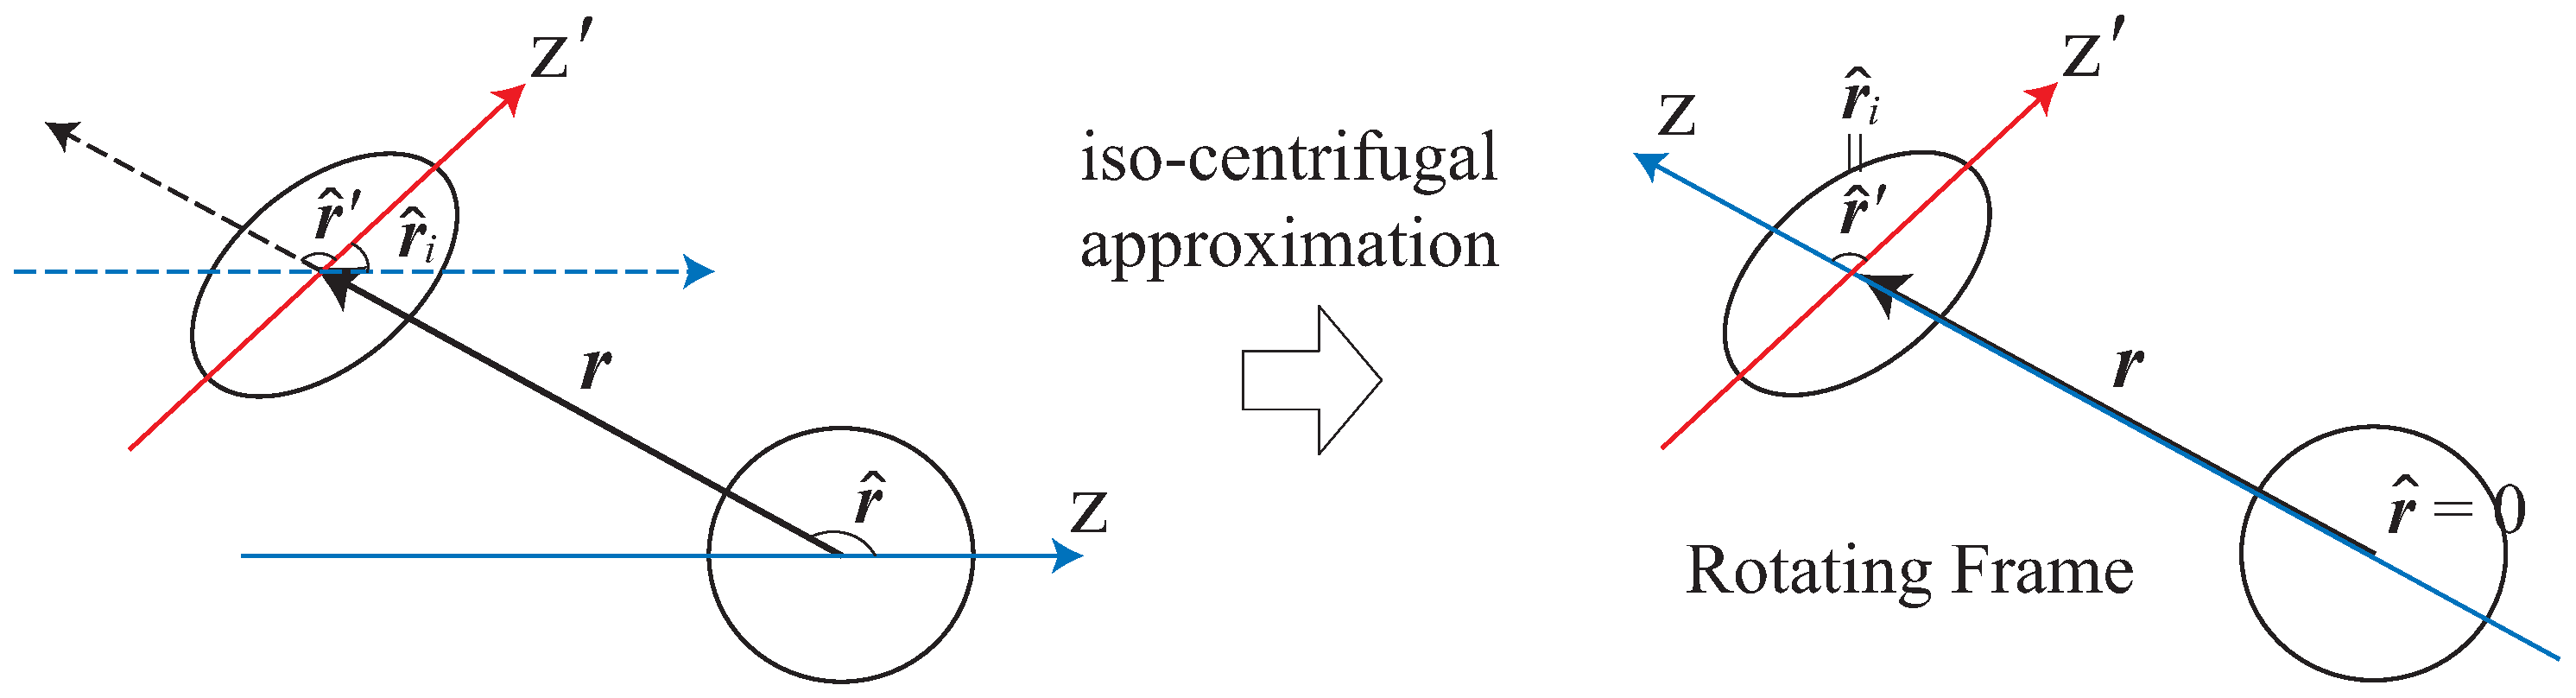
\includegraphics[clip,keepaspectratio,height=42mm]{figure/chapter3/isocent.eps}
  \caption{The angles in the original coordinate systems(left), 
           and those in the iso-centrifugal approximations(right).}
  \label{fig3.00}
\end{figure}
On the other hand, the differential cross sections for the channel $(n,I)$ are
given by
\begin{eqnarray}
\frac{d\sigma_{nI}}{d\Omega} = \frac{k_{nI}}{k_{n_iI_i}}|f_{nI,n_iI_i}(\theta)|^2
\end{eqnarray}
with the scattering amplitude
\begin{eqnarray}
f_{nI,n_iI_i}(\theta) &=& \frac{1}{2i\sqrt{k_{n_iI_i}k_{nI}}}\sum_{J} 
e^{i\left[\sigma_{J}(E)+\sigma_{J}(E-\epsilon_{nI})\right]}
(2J+1)P_{J}({\rm cos}\theta)
(S_{nI,n_iI_i}^{J} - \delta_{n,n_i}\delta_{I,I_i}) \\ \nonumber
&& + f_{\rm C}(\theta)\delta_{n,n_i}\delta_{I,I_i}, 
\end{eqnarray}
where $\sigma_{J}(E)$ and $f_{\rm C}(\theta)$ are the Coulomb phase shift and
the Coulomb scattering amplitude, respectively.
The quasi-elastic scattering cross section is then 
defined by the sum of the elastic and the inelastic cross sections, that is,
\begin{eqnarray}
\frac{d\sigma_{\rm qel}}{d\Omega}
= \sum_{n,I}\frac{d\sigma_{nI}}{d\Omega}.
\end{eqnarray}

The iso-centrifugal approximation has been found to be a good approximation for
heavy-ion reactions~\cite{T87}.
In order to see the validity of this approximation, we consider the fusion reaction
of $^{24}$Mg + $^{90}$Zr system.
We take into account rotational excitations of $^{24}$Mg up to the $4^+$ state with
the excitation energy $\epsilon_2 = 1.37$ MeV and the deformation parameter
$\beta_2 = 0.505$.
In this case, for $J \ge 4$, 
the dimension of the coupled-channels equations in the full angular
coupling scheme amounts to 9
[$(I,\ell) =
(0,J),(2,J),(4,J),(2,J\pm2),(4,J),(4,J\pm2),(4,J\pm4)$],
while it reduces to 3 $[I = 0, 2, 4]$ in the iso-centrifugal
approximation. If one takes into account two more rotational states
up to the $8^+$ state,
the number of the coupled-channels equations in the full angular coupling becomes 25.

In Fig.\ref{fig3.0}, we show the result of numerical calculation.
The solid blue lines and the red dashed lines show the result with and
without the iso-centrifugal approximation, respectively. Fig.\ref{fig3.0}(a) and
(b) show the fusion cross section in the linear and logarithmic scales, respectively
and Fig.\ref{fig3.0}(c) represents the fusion barrier distribution defined
in Sec.3.4.
Although one can observe some discrepancy between the two calculations for fusion
cross sections above the barrier and the fusion barrier distribution, the difference 
is rather
small. This comparison shows the validity of the iso-centrifugal
approximation.
\begin{figure}[t]
  \center
  \includegraphics[clip,keepaspectratio,width=80mm]{figure/chapter3/fus_24Mg_90Zr_iso_cent.pdf}
  \caption{Fusion cross sections and fusion barrier distribution for $^{24}$Mg +
  $^{90}$Zr system. Fig. \ref{fig3.0}(a) and \ref{fig3.0}(b)
  show the fusion cross section in the linear and
  logarithmic scales, respectively and Fig. \ref{fig3.0}(c) 
  represents the fusion barrier
  distribution. The red dashed lines represent the result in the full angular
  coupling while the blue solid lines represent the result in the
  iso-centrifugal approximation.}
  \label{fig3.0}
\end{figure}

\section{Sudden tunneling limit}
We have now obtained the coupled-channels equations to be solved.
In the following, we shall see the consequence of the channel coupling.
First we consider the case where the excitation energies are neglected.
We assume that only a single mode
with $\lambda$ in the coupling Hamiltonian is involved for simplicity.
In this case, one can diagonalize the coupling matrix with a coordinate
independent matrix and decouple the coupled-channels equations.
The approximation neglecting the excitation energies is
referred to as the sudden tunneling
approximation and corresponds to assuming that 
the tunneling process occurs much faster than
the internal motion of the colliding nuclei.
Here, we show that the coupled-channels equations are decoupled in this limit
and the concept of the barrier distributions naturally appears.

The coupled-channels equations in the sudden tunneling limit are given by
\begin{eqnarray}
\left[-\frac{\hbar^2}{2\mu}\frac{d^2}{dr^2}
+ \frac{J(J+1)\hbar^2}{2\mu r^2} + V_0(r) - E\right]
u_{n}^J(r)
= - \sum_{n^\prime}
\sqrt{\frac{2\lambda+1}{4\pi}}
f_{\lambda}(r)
\left\langle \phi_{n} \left|T_{\lambda 0}
\right| \phi_{n^\prime} \right\rangle
u_{n^\prime}^J(r),
\end{eqnarray}
where, the label of the intrinsic spin $I$ are omitted for simplicity.
One can diagonalize the coupling matrix
\begin{eqnarray}
V_{nm}(r) = \sqrt{\frac{2\lambda+1}{4\pi}}f_{\lambda}(r)
\langle \phi_n | T_{\lambda0} | \phi_m \rangle
\end{eqnarray}
with a coordinate independent matrix $U$ which diagonalizes the matrix
$\langle \phi_n | T_{\lambda0} | \phi_m \rangle$, that is,
\begin{eqnarray}
U^{\dagger}VU = diag\left\{\lambda_1(r),\lambda_2(r), \cdots,
\lambda_N(r)\right\}.
\end{eqnarray}
Here, $N$ stands for the dimension of the coupled-channels equations.
Each eigenvalue of $V$ is given by the product of the eigenvalue of the matrix
$\displaystyle \sqrt{\frac{2\lambda+1}{4\pi}}\langle \phi_n | T_{\lambda0} | \phi_m \rangle$ and $f_{\lambda}(r)$.
The coupled-channels equations are then transformed to
\begin{eqnarray}
\left[-\frac{\hbar^2}{2\mu}\frac{d^2}{dr^2}
+ \frac{J(J+1)\hbar^2}{2\mu r^2} + V_0(r) + \lambda_{\alpha}(r) - E\right]
v_{\alpha}^J(r)
= 0.
\end{eqnarray}
Here, $\bvec{v}^J(r) = U^{\dagger}\bvec{u}^J(r)$,
or $\displaystyle v_{\alpha}^J(r) = \sum_n U_{n\alpha}^{*}(r) u_n^J(r)$.
We call the channel $\alpha$ in this representation an eigenchannel and the
potential barrier given by $V(r) + \lambda_{\alpha}(r)$ an eigenbarrier.
The boundary condition for $v_{\alpha}(r)$ now reads
\begin{align}
v_{\alpha}^J(r) &\rightarrow \sum_n U_{n_i\alpha}^{*}
\left\{H_J^{(-)}(k_{n_i}r)\delta_{n,n_i} - S_{nn_i}^J H_J^{(+)}(k_nr)\right\} \\
&= U_{n_i\alpha}^{*}\left\{H_J^{(-)}(k_{n_i}r) 
- \tilde{S}_{\alpha n_i}^J H_J^{(+)}(k_nr) \right\}
\end{align}
for $r \rightarrow \infty$. Here, we have removed a factor
$\displaystyle \sqrt{\frac{k_{n_i}}{k_n}}$ because it equals to unity in the sudden 
tunneling limit, and $\tilde{S}_{\alpha n_i}^J$ is defined by
\begin{eqnarray}
\tilde{S}_{\alpha n_i}^J = \sum_n \frac{U_{n\alpha}^{*}}{U_{n_i\alpha}^{*}}
S_{nn_i}^J.
\end{eqnarray}
By taking an absolute square of the both hand sides of 
$\displaystyle U_{n_i\alpha}^{*}\tilde{S}_{\alpha n_i}^J = \sum_nU_{n\alpha}^{*}S_{nn_i}^J$
and summing over $\alpha$, one can show
\begin{eqnarray}
\sum_n \left|S_{nn_i}^J \right|^2
= \sum_{\alpha}\left|U_{n_i\alpha}\right|^2 \left| \tilde{S}_{\alpha n_i}^J\right|^2.
\end{eqnarray}
Substitution of the above relation to Eq. (\ref{fus_cs}) gives
\begin{eqnarray}
\sigma_{\rm fus}(E)
= \sum_{\alpha} w_{\alpha} \sigma_{\rm fus}^{(\alpha)}(E)
\label{fus_sudden}
\end{eqnarray}
with the weight factor $w_{\alpha} = |U_{n_i\alpha}|^2$ and the fusion cross
section for eigenchannel $\alpha$
\begin{eqnarray}
\sigma_{\rm fus}^{(\alpha)}(E) = \frac{\pi}{k_0^2}
\sum_J(2J+1)\left(1 - \left| \tilde{S}_{\alpha n_i}^J\right|^2\right),
\end{eqnarray}
where $\displaystyle k_0 = \sqrt{\frac{2\mu E}{\hbar^2}}$.
Similarly, one can show
\begin{eqnarray}
S_{nn_i}^J = \sum_{\alpha}U_{n_i\alpha}^{*} U_{n\alpha}\tilde{S}_{\alpha n_i}^J,
\end{eqnarray}
and correspondingly, the scattering amplitude is now written as
\begin{eqnarray}
f_{n}(\theta) = \sum_{\alpha} U_{n_i\alpha}^{*}
U_{n\alpha}\tilde{f}_{\alpha}(\theta)
\end{eqnarray}
with
\begin{eqnarray}
\tilde{f}_{\alpha}(\theta)
= \frac{1}{2ik_0}\sum_J e^{2i\sigma_J} (2J+1) P_J({\rm cos}\theta)
\left(S_{\alpha n_i}^J - 1\right) + f_{\rm C}(\theta).
\end{eqnarray}
The quasi-elastic scattering cross sections are represented as
\begin{eqnarray}
\frac{d\sigma_{\rm qel}}{d\Omega} = \sum_{\alpha} w_{\alpha}
\frac{d\sigma_{\rm el}^{(\alpha)}}{d\Omega}
=\sum_{\alpha} w_{\alpha} \left| \tilde{f}_{\alpha}(\theta)\right|^2.
\end{eqnarray}
From these expressions, one can see that both the fusion cross sections and the
quasi-elastic cross sections are given by the weighted sum of the cross sections
over the eigenchannels in the sudden tunneling limit.
Some eigenchannels have the barrier lower than the original Coulomb barrier,
and the others have higher ones.
This leads to the concept of the barrier distribution for the fusion reaction and
the quasi-elastic scattering. 
In the following section, we explain how the barrier distribution is extracted
from experimental fusion and quasi-elastic cross sections.

\section{Barrier distribution method}
In order to get further understanding of the experimental data for heavy-ion
reactions, Rowley, Satchler, 
and Stelson introduced a method to extract distribution of
barriers directly from the experimental fusion cross sections\cite{fusionbar}.
To illustrate the method, let us consider the classical expression for the
fusion cross section. It is given by
\begin{eqnarray}
\sigma_{\rm fus}^{cl}(E)
= \pi R_{\rm B}^2 \left(1 - \frac{V_{\rm B}}{E}\right)\theta(E-V_{\rm B}),
\end{eqnarray}
where $V_{\rm B}$ is the Coulomb barrier height and $R_{\rm B}$ is the
barrier radius, that is $V(r = R_{\rm B}) = V_{\rm B}$. $\theta(x)$ is the step
function. For a derivation of this equation, see Appendix A.
From this expression, one can immediately get the classical barrier penetrability by
\begin{eqnarray}
\frac{1}{\pi R_{\rm B}^2}\frac{d(E\sigma_{\rm fus}^{cl})}{dE} = \theta(E-V_{\rm B}),
\label{eq3.35}
\end{eqnarray}
and the derivative of the penetrability gives a delta function which has a peak at
$E = V_{\rm B}$. 
In quantum mechanics, the quantum tunneling effect smears the
delta function.
For example, if one approximates the potential barrier by a parabolic potential,
$V(r) \approx V_{\rm B} - \displaystyle \frac{1}{2}\mu\Omega^2(r - R_{\rm B})^2$,
the fusion cross sections are given by the following Wong formula\cite{Wong}
\begin{eqnarray}
\sigma_{\rm fus}(E) = \frac{\hbar\Omega R_{\rm B}^2}{2E}{\rm ln}
\left\{1 + {\rm exp}\left[(2\pi/\hbar\Omega)(E-V_{\rm B})\right]\right\},
\end{eqnarray}
and the second derivative of $E\sigma_{\rm fus}$ gives
\begin{eqnarray}
\frac{1}{\pi R_{\rm B}^2}\frac{d^2(E\sigma_{\rm fus})}{dE^2}
= \frac{2\pi}{\hbar\Omega}\frac{e^x}{(1+e^x)^2},
\label{bd_Wong}
\end{eqnarray}
where $x = (2\pi/\hbar\Omega)(E - V_{\rm B})$.
This quantity is called the fusion barrier distribution and has a peak at
$E = V_{\rm B}$. We show in Fig. \ref{Wong1}
the fusion cross sections and the fusion
barrier distribution of the Wong formula for $^{20}$Ne + $^{90}$Zr system.
The height, position, and curvature of the Coulomb barrier are
$V_{\rm B} = 52.0$ MeV, $R_{\rm B} = 10.4$ fm, and
$\hbar\Omega =$ 4.05 MeV, respectively.
For comparison, the
classical fusion cross sections are also shown by the dotted line.
The width of the barrier distribution is related to the curvature of the
parabola, that is, the full width half maxima(FWHM) is given by $0.56\hbar\Omega$.
For the detail, see appendix A.

\begin{figure}[t]
  \begin{center}
    \begin{minipage}[t]{80mm}
      \includegraphics[clip,keepaspectratio,width=80mm]{figure/chapter3/fusion_Wong2.eps}
      \caption{The upper panel: Fusion cross sections for $^{20}$Ne + $^{90}$Zr 
      system from the Wong formula (the red solid line). 
      The black dotted line is the classical fusion cross sections.
      The lower panel: Corresponding fusion barrier distribution
      defined by Eq. (\ref{bd_Wong}).}
      \label{Wong1}
    \end{minipage}
  \end{center}
\end{figure}

In the previous section, we have seen that the fusion cross sections are give by
the weighted sum of the fusion cross sections over the eigenchannels in the
sudden tunneling limit. By taking the second derivative of
the product of $E$ and the both hand sides of
Eq. (\ref{fus_sudden}), we get
\begin{eqnarray}
D_{\rm fus}(E) = 
\frac{1}{\pi R_{\rm b}^2} \frac{d^2(E\sigma_{\rm fus})}{dE^2}
= \sum_{\alpha}w_{\alpha}
\frac{1}{\pi R_{\rm b}^2} \frac{d^2(E\sigma_{\rm fus}^{(\alpha)})}{dE^2}.
\end{eqnarray}
Each term in the sum has a peak at the position of the eigenbarrier, and the 
$D_{\rm fus}(E)$ is given by the weighted sum of them.
Thus, the $D_{\rm fus}(E)$ represents a distribution of eigenbarriers and is
called fusion barrier distribution.
Rowley {\it et al.} proposed that one can extract the fusion barrier
distribution from measured fusion cross sections $\sigma_{\rm
fus}(E)$\cite{fusionbar}.
Compared to the fusion cross sections themselves, the fusion barrier
distribution more clearly indicates the effect of the coupling.
In fact, it can serve for the determination of deformation
parameters\cite{LRL93}.
Note that although the fusion cross section contains the contributions from all
partial waves, the differentiation of it gives the penetrability of the
potential for s-wave as can be seen from Eq. (\ref{eq3.35}).

In the actual calculation of the fusion barrier distribution 
from the fusion cross sections, one
replaces the differentiation with finite difference, that is,
the value of the barrier distribution at energy $(E_1 + 2E_2+E_3)/4$ is
calculated as
\begin{eqnarray}
\frac{d^2(E\sigma_{\rm fus})}{dE^2}
=2\left(\frac{(E\sigma_{\rm fus})_3 - (E\sigma_{\rm fus})_2}{E_3 - E_2}
 - \frac{(E\sigma_{\rm fus})_2 - (E\sigma_{\rm fus})_1}{E_2 - E_1}
 \right)
 \left(\frac{1}{E_3 - E_1}\right),
\end{eqnarray}
where $(E\sigma_{\rm fus})_i$ are evaluated at energies $E_i$.
If one uses equal energy intervals $\Delta E = (E_2 - E_1) = (E_3 - E_2)$,
this reduces to
\begin{eqnarray}
\frac{d^2(E\sigma_{\rm fus})}{dE^2}
= \left(
\frac{(E\sigma_{\rm fus})_3 - 2(E\sigma_{\rm fus})_2 + (E\sigma_{\rm
fus})_1}{\Delta E^2}\right).
\end{eqnarray}
The error $\delta_c$ is estimated as\cite{dasgupta}
\begin{eqnarray}
\delta_c \approx \left(\frac{E}{\Delta E^2}\right)
\sqrt{
(\delta\sigma_{\rm fus}^2)_1^2 + 4(\delta\sigma_{\rm fus})_2^2
+ (\delta\sigma_{\rm fus})_3^2}.
\end{eqnarray}
The value of $\Delta E$ is usually taken about 2 MeV in the center-of-mass frame.
For calculations presented in this thesis, $\Delta E = 2$ MeV is always adopted.

A similar concept has been also applied to the quasi-elastic scattering
\cite{timmers, HR04}.
As in the case of fusion reaction, let us first consider the classical
expression for scattering. In the limit of the strong Coulomb field, the elastic
scattering cross section at $\theta = \pi$ is given by
\begin{eqnarray}
\sigma_{\rm el}^{cl}(E,\pi) = \sigma_{\rm R}(E,\pi)\theta(V_{\rm B} - E),
\end{eqnarray}
where $\sigma_{\rm R}(E,\theta)$ is the Rutherford cross section.
Thus,
$\sigma_{\rm el}^{cl}(E,\pi) / \sigma_{\rm R}(E,\pi)$ equals to
$\theta(V_{\rm B} - E)$
and this corresponds to the reflection probability.
By differentiating it with respect to energy, one gets
\begin{eqnarray}
D_{\rm qel}(E,\pi) = - \frac{d(\sigma_{\rm qel}(E,\pi)/\sigma_{\rm R}(E,\pi))}{dE} = \delta(E - V_{\rm B}).
\end{eqnarray}
Since in the sudden tunneling limit, 
the quasi-elastic cross sections are represented by the weighted sum of
the elastic cross sections over the eigenchannels as in the fusion case,
$D_{\rm qel}(E,\pi)$ also gives the distribution of eigenbarriers.
Although the discussion here assumed a strong Coulomb field in the scattering,
the nuclear effect has to be taken into account for realistic systems.
In fact, the elastic cross section deviates from the Rutherford cross section
as the incident energy increases (cf. Fig. \ref{potential}).
Nevertheless, the quasi-elastic barrier distribution
exhibits a similar behavior to the
fusion barrier distribution, although the quasi-elastic barrier distribution is
usually more smeared\cite{timmers,HR04,zamrun}.
In Fig. \ref{fus_and_qel}, we show the comparison of the fusion and the
quasi-elastic barrier distributions for $^{24}$Mg + $^{90}$Zr system.
The red solid line represents the fusion barrier distribution and the blue
dashed line represents the quasi-elastic barrier distribution.
The upper panel is for the calculation without channel coupling
and the lower panel is for the calculation 
which includes the rotational excitations of $^{24}$Mg up to
$4^+$ state.
All of the barrier distributions are normalized to unit area
in the energy interval between 50 and 75 MeV.
One can see that the quasi-elastic barrier distribution of the single-channel
calculation exhibits more asymmetric
behavior compared to that of the fusion,
that is, it possesses a moderate tail
at the lower energy side.
However, the behavior of the both barrier distributions is quite similar, while the
peaks in the quasi-elastic barrier distribution are somewhat smaller than those
of the fusion case.
In evaluating the quasi-elastic barrier distribution,
we replace the differentiation by finite difference as in the fusion barrier distribution.
The energy interval $\Delta E$ is taken to be 2 MeV in our calculations in this
thesis.
\begin{figure}[t]
  \begin{center}
    \begin{minipage}[t]{100mm}
      \includegraphics[clip,keepaspectratio,width=100mm]{figure/chapter3/fusion_and_qel.pdf}
      \caption{Comparison of the fusion(the red solid line) and
      the quasi-elastic(the blue dashed line)
      barrier distributions for $^{24}$Mg + $^{90}$Zr system. They are
      normalized to unity if integrated over the energy.}
      \label{fus_and_qel}
    \end{minipage}
  \end{center}
\end{figure}


In actual experiments, detection of the scattered particle at $\theta = \pi$ is
impossible.
However, one can correct the effect of the difference in the detection angles by
subtracting the centrifugal energy from the incident energy.
Estimating the centrifugal potential at the Coulomb turning point $r_{\rm c}$,
the effective energy is given by
\begin{eqnarray}
E_{\rm eff} = E - \frac{\lambda_{\rm c}^2\hbar^2}{2\mu r_{\rm c}^2}
= 2E\frac{{\rm sin}\frac{\theta}{2}}{1+{\rm sin}\frac{\theta}{2}},
\label{effective_E}
\end{eqnarray}
where, $\lambda_{\rm c} = \displaystyle \eta {\rm cot}\frac{\theta}{2}$ with $\eta$
being the Sommerfeld parameter, and $r_{\rm c}$ is defined by
$\displaystyle E = \frac{Z_{\rm P}Z_{\rm T}e^2}{r_{\rm c}} + \frac{\lambda_{\rm
c}^2\hbar^2}{2\mu r_{\rm c}^2}$.

While one has to take a second derivative of $E\sigma_{\rm fus}$ to extract
the fusion barrier distribution, one can get the quasi-elastic barrier
distribution by differentiating $\sigma_{\rm qel}/\sigma_{\rm R}$ one
time.
As mentioned above, the scattering angle is classically related
to the orbital angular momentum.
Therefore, by choosing the scattering at $\theta=\pi$, one can attain the
penetrability for s-wave without differentiation. 

We have introduced the barrier distribution method
based on the eigenchannel representation in the sudden tunneling limit.
However, the concept of the barrier distribution has been found to be valid
even if the finite excitation energy is taken into account.
In that case, the weight factors in the eigenchannel representation become
energy dependent and change slowly with the energy\cite{HTB97}.




\section{Constant coupling approximation}
In the previous section, we have seen that the eigenchannel representation in
the sudden tunneling limit leads to
the barrier distribution method.
The eigenchannel representation
can be introduced also when
the coupling matrix is
coordinate independent. This approximation is called 
a constant coupling approximation\cite{DLW83}.
In this approximation,
the coupled-channels equations read
\begin{align}
\left[-\frac{\hbar^2}{2\mu}\frac{d^2}{dr^2}
+ \frac{J(J+1)\hbar^2}{2\mu r^2} + V_0(r) - E\right]
&u_{n}^J(r) \nonumber\\
= - \sum_{m}
&\left[
\epsilon_n \delta_{n,m} +
\sum_{\lambda}
\sqrt{\frac{2\lambda+1}{4\pi}}
f_{\lambda}^0
\left\langle \phi_{n} \left|T_{\lambda 0}
\right| \phi_{m} \right\rangle
\right]u_{m}^J(r),
\end{align}
where, $f^0_{\lambda}$ is a constant.
One can diagonalize the matrix 
\begin{eqnarray}
V_{nm} = 
\epsilon_n \delta_{n,m} +
\sum_{\lambda}
\sqrt{\frac{2\lambda+1}{4\pi}}
f_{\lambda}^0
\left\langle \phi_{n} \left|T_{\lambda 0}
\right| \phi_{m} \right\rangle
\end{eqnarray}
with a coordinate independent matrix as in the case of the sudden tunneling
limit, and the fusion and the quasi-elastic cross sections are given by the
weighted sum of the cross sections over the eigenchannels.


\section{Coupling to collective states}
In this section, coupling effects to collective excited states are reviewed.
\subsection{Vibrational coupling}
First we consider the vibrational coupling for a projectile nucleus.
As seen in chapter 2, in the liquid drop model, the shape of the nuclear
surface is parametrized as
\begin{eqnarray}
R = R_{\rm P} \left(
1 + \sum_{\lambda}\alpha_{\lambda}\cdot Y_{\lambda}
\right).
\end{eqnarray}
In the following discussion, we consider a particular mode $\lambda$.
The Hamiltonian for the vibration is given by (\ref{collham}).
After quantization procedure, the Hamiltonian is represented as
\begin{eqnarray}
H = \sum_{\mu}\frac{1}{2}\hbar\omega_{\lambda}b_{\lambda\mu}^{\dagger}b_{\lambda\mu},
\end{eqnarray}
where, $\omega_{\lambda}=\sqrt{C_{\lambda}/B_{\lambda}}$, and the zero-point
energy is removed.
The creation and the annihilation operators $b_{\lambda\mu}^{\dagger}$ 
and $b_{\lambda\mu}$ are related with $\alpha_{\lambda\mu}$ by
\begin{eqnarray}
\alpha_{\lambda\mu} = \sqrt{\frac{\hbar}{2B_{\lambda}\omega_{\lambda}}}
\left(b_{\lambda\mu}^\dagger + (-1)^\mu b_{\lambda\mu} \right).
\label{alpha_b1}
\end{eqnarray}
The deformation parameter for the 
vibration with $\lambda$ is defined by the square
root of the amplitude of the zero-point vibration, that is,
\begin{align}
\beta_{\lambda}^2 &= \langle n_{\lambda} = 0 |
\sum_{\mu}\alpha_{\lambda\mu}^{\dagger}\alpha_{\lambda\mu}|
n_{\lambda} = 0 \rangle \\
&= (2\lambda+1)\frac{\hbar}{2B_{\lambda}\omega_{\lambda}}.
\end{align}
Thus, Eq. (\ref{alpha_b1}) is rewritten as
\begin{eqnarray}
\alpha_{\lambda\mu} = \frac{\beta_{\lambda}}{\sqrt{2\lambda+1}}
\left(b_{\lambda\mu}^\dagger + (-1)^\mu b_{\lambda\mu} \right).
\label{alpha_b2}
\end{eqnarray}
The nuclear potential between the colliding nuclei is given by a function of
the distance between the nuclear surface points on a line connecting the center
of each nucleus.
For spherical nuclei with the radius $R_{\rm T}$ and $R_{\rm P}$,
the distance is given by $r - R_{\rm T} - R_{\rm P}$.
If one takes into account the coupling of the projectile, the nuclear potential is
obtained by replacing $r-R_{\rm T}-R_{\rm P}$ by
$r -  R_{\rm T} - R_{\rm P} - R_{\rm P}\alpha_{\lambda}\cdot Y_{\lambda}$,
that is, the nuclear potential $V_{\rm N}(r)$ is replaced by $
V_{\rm N}(r - R_{\rm P}\alpha_{\lambda}\cdot
Y_{\lambda}(\hat{\bvec{r}}))$.
In order to extract a form factor of the coupling Hamiltonian, let us assume
that the $\beta_{\lambda}$ is small and expand the potential up to the first
order term with respect to $\beta_{\lambda}$ 
(the linear coupling approximation)
\begin{align}
V_{\rm N}\left(r - R_{\rm P}\alpha_{\lambda}\cdot
Y_{\lambda}(\hat{\bvec{r}})
\right)
&\approx V_{\rm N}(r) - R_{\rm P}\frac{dV_{\rm N}(r)}{dr}
\alpha_{\lambda}\cdot Y_{\lambda}(\hat{\bvec{r}}).
\end{align}
The second term gives the nuclear part of the coupling Hamiltonian.

Next we consider the Coulomb part of the coupling Hamiltonian.
Let us denote the density of the vibrating projectile by $\rho_{\rm P}(\bvec{r})$.
Then, the Coulomb potential between the colliding nuclei is given by
\begin{eqnarray}
V_{\rm C}(\bvec{r}) = \int d\bvec{r}^\prime
\frac{Z_{\rm P}Z_{\rm T}e^2}
{|\bvec{r} - \bvec{r}^\prime|}
\rho_{\rm P}(\bvec{r}^\prime)
\end{eqnarray}
for $\bvec{r}$ larger than the range of $\rho_{\rm P}(\bvec{r})$.
By using the expansion formula
\begin{eqnarray}
\frac{1}{
|\bvec{r} - \bvec{r}^\prime|}
= \sum_{\lambda^\prime\mu^\prime}
\frac{4\pi}{2\lambda^\prime + 1}
\frac{r_<^{\lambda^\prime}}{r_>^{\lambda^\prime+1}}
Y_{\lambda^\prime\mu^\prime}(\hat{\bvec{r}}^\prime)
Y_{\lambda^\prime\mu^\prime}^{*}(\hat{\bvec{r}}),
\end{eqnarray}
the potential is represented as
\begin{eqnarray}
V_{\rm C}(\bvec{r}) = 
\frac{Z_{\rm P}Z_{\rm T}e^2}{r}
+ \sum_{\lambda^\prime > 0} \sum_{\mu^\prime}
\frac{4\pi Z_{\rm T}e}{2\lambda^\prime+1}
Q_{\lambda\mu^\prime}
Y_{\lambda^\prime\mu^\prime}^{*}(\hat{\bvec{r}})
\frac{1}{r^{\lambda^\prime+1}},
\end{eqnarray}
where, the electric multipole operator is defined as
\begin{eqnarray}
Q_{\lambda\mu}
= \int d\bvec{r}
Z_{\rm P}e\rho_{\rm P}(\bvec{r})
r^{\lambda} Y_{\lambda\mu}(\hat{\bvec{r}}).
\end{eqnarray}
Assuming a sharp distribution for $\rho_{\rm P}(\bvec{r})$, that is,
\begin{eqnarray}
\rho_{\rm P}(\bvec{r}) = \rho_0 \theta(R(\theta,\phi) - r),\ \ \ \ 
\rho_0 = \frac{3}{4\pi R_{\rm P}^3},
\end{eqnarray}
$Q_{\lambda^\prime\mu^\prime}$ is given by
\begin{eqnarray}
Q_{\lambda^\prime\mu^\prime} = \frac{3Z_{\rm P}e}{4\pi}
R_{\rm P}^\lambda\alpha_{\lambda\mu^\prime}\delta_{\lambda\lambda^\prime}
\label{multipole_op}
\end{eqnarray}
up to the first order in $\alpha_{\lambda\mu}$.
Thus, the Coulomb potential reads
\begin{eqnarray}
V_{\rm C}(\bvec{r}) = 
\frac{Z_{\rm P}Z_{\rm T}e^2}{r}
+
\frac{3}{2\lambda+1}Z_{\rm P}Z_{\rm T}e^2
\frac{R_{\rm P}^\lambda}{r^{\lambda+1}}
\alpha_{\lambda}\cdot Y_{\lambda}(\hat{\bvec{r}}),
\end{eqnarray}
and the second term gives the Coulomb part of the coupling Hamiltonian.

Combining the nuclear and the Coulomb potentials, the coupling Hamiltonian is given
by
\begin{eqnarray}
V_{\rm coup}(\bvec{r},\alpha_{\lambda\mu})
= f_{\lambda}(r)\alpha_{\lambda}\cdot Y_{\lambda}(\hat{\bvec{r}})
\end{eqnarray}
with the form factor
\begin{eqnarray}
f_{\lambda}(r)
=
- R_{\rm P}\frac{dV_{\rm N}(r)}{dr}
+ \frac{3}{2\lambda+1}Z_{\rm P}Z_{\rm T}e^2
  \frac{R_{\rm P}^\lambda}{r^{\lambda+1}}.
\label{vib_form_factor}
\end{eqnarray}
Under the iso-centrifugal approximation, $V_{\rm coup}$ becomes
\begin{align}
V_{\rm coup}(\bvec{r}, \alpha_{\lambda\mu})
&= f_{\lambda}(r) \alpha_{\lambda}\cdot Y_{\lambda}(\hat{\bvec{r}} = 0) 
\nonumber \\
&= \frac{\beta_{\lambda}}{\sqrt{4\pi}}
  f_{\lambda}(r)(b_{\lambda 0}^{\dagger} + b_{\lambda 0}).
\label{Vcoup_vib}
\end{align}
At the position of the barrier $R_{\rm B}$, it holds that
$dV_0/dr = dV_{\rm N}/dr + dV_{\rm C}/dV = 0$,
that is,
\begin{eqnarray}
   -\left.\frac{dV_{\rm N}}{dV}\right|_{r=R_{\rm B}}
= - \left.\frac{Z_{\rm P}Z_{\rm T}e^2}{r^2}\right|_{r=R_{\rm B}}.
\end{eqnarray}
The form factor $f_{\lambda}(r)$ is then estimated
at $r = R_{\rm B}$ as
\begin{eqnarray}
f_{\lambda}(R_{\rm B}) = -R_{\rm P} \frac{Z_{\rm P}Z_{\rm T}e^2}{R_{\rm B}^2}
+ \frac{3}{2\lambda+1}Z_{\rm P}Z_{\rm T}e^2
  \frac{R_{\rm P}^\lambda}{R_{\rm B}^{\lambda+1}}.
\end{eqnarray}
One can see that the form factor is proportional to the charge product.
Therefore, the coupling strength is effectively stronger for systems which have
a larger charge product.

Although the coupled-channels equations (\ref{cc_iso}) use the basis
where the intrinsic spin $I$ is a good quantum number,
it is more efficient to work in another basis
for the vibrational excitations in the iso-centrifugal approximation\cite{KRNR93}.
Let us first consider 1-phonon states. They are given by
$\left\{b_{\lambda\mu}^{\dagger}|0\rangle\right\}_{\mu}$ and these states span
the $(2\lambda+1)$-dimensional subspace.
Among them, only a state $b_{\lambda 0}^{\dagger}|0\rangle$ can be excited
from the ground state by $V_{\rm coup}$ given in (\ref{Vcoup_vib}).
Thus, it is sufficient to take into account only one channel for 1-phonon
states.

Next consider 2-phonon states.
They are given by
$\left\{[b_{\lambda}^{\dagger}b_{\lambda}^{\dagger}]^{(IM)}|0\rangle\right\}_{IM}$.
For $\lambda=2$ case, the possible values of $I$ are 0, 2, and 4, and the states
$(0^+,2^+,4^+)$ form a triplet with the same excitation energy. The dimension of
the subspace spanned by the 2-phonon states is 15.
The set
$\left\{[b_{\lambda}^{\dagger}b_{\lambda}^{\dagger}]^{(IM)}|0\rangle\right\}_{IM}$
can be unitary transformed to a set
$\left\{b_{\lambda\mu}^{\dagger}b_{\lambda\mu^\prime}^{\dagger}|0\rangle\right\}_{\mu\mu^\prime}$.
Among them, in the iso-centrifugal approximation, only the state
$b_{\lambda 0}^{\dagger}b_{\lambda 0}^{\dagger}|0\rangle$
can be excited from the 1-phonon state $b_{\lambda 0}^{\dagger}|0\rangle$ by $V_{\rm
coup}$.
Thus, it is sufficient to take into account only one channel for 2-phonon
states.
One can progress this discussion to $n$-phonon states, and will find that
only one channel is necessary to represent $n$-phonon states
in the iso-centrifugal approximation.
Therefore, the total basis is given by
$\left\{\displaystyle \frac{1}{\sqrt{n!}}\left(b_{\lambda 0}^{\dagger}\right)^n
|0\rangle\right\}_n$.
The coupling matrix element between $n$-phonon channel and $m$-phonon channel is
then given by
\begin{eqnarray}
V_{nm}(r) = \frac{\beta_{\lambda}}{\sqrt{4\pi}}f_{\lambda}(r)
\left(
\delta_{n,m-1}\sqrt{m} + \delta_{n,m+1}\sqrt{n}
\right),
\end{eqnarray}
and the matrix is given by
\begin{eqnarray}
\displaystyle
(V_{nm})  = \frac{\beta_{\lambda}}{\sqrt{4\pi}}f_{\lambda}(r)
      \left(
        \begin{array}{ccc}
          0  &  1 & 0        \\
          1  &  0 & \sqrt{2} \\
          0  &  \sqrt{2}  & 0
        \end{array}
      \right),
\end{eqnarray}
if one truncates the space up to the 2-phonon channel.

As an example of the vibrational coupling, we show in Fig. \ref{fig3.1} 
the calculation of the fusion reaction for
$^{32}$S + $^{90}$Zr system.
\begin{figure}[t]
  \center
  \includegraphics[clip,keepaspectratio,width=85mm]{figure/chapter3/fus_32S_90Zr_coll_32S.eps}
  \caption{Fusion cross sections and fusion barrier distribution for $^{32}$S +
  $^{90}$Zr system. The black dotted lines show the calculation without the
  channel coupling, the red solid lines take into account the vibrational
  excitation of $^{32}$S up to the 1-phonon state, and the blue solid lines take
  into account the vibrational excitations up to the 2-phonon state.}
  \label{fig3.1}
\end{figure}
Figs.\ref{fig3.1}(a) and \ref{fig3.1}(b) show the fusion cross sections in
the linear and logarithmic scales, respectively.
Fig.\ref{fig3.1}(c) shows the fusion barrier distribution.
The black dotted lines show the calculation without coupling, the red solid
lines take into account the vibrational quadrupole excitations of $^{32}$S up to
the one-phonon state, and the blue solid lines includes up to the two-phonon state.
The excitation energy and the deformation parameter
of the $2^{+}$ state of $^{32}$S
are $\epsilon_2$ = 2.23 MeV and $\beta_2$ = 0.32, respectively.
These calculations include the contribution from all order terms in $\beta_2$ in
the nuclear coupling (See Sec.3.7).
In the absence of the coupling, the barrier distribution shows a single peak at
the Coulomb barrier ($V_{\rm B}=82.5$ MeV).
One can see that by including the coupling,
the subbarrier fusion cross sections
are enhanced (Fig. \ref{fig3.1}(b)),
and the potential barrier distributes in energy.
In the case the vibrational coupling,
the lower barrier is taller than the higher one.

%Note that one should take into account more relevant collective excitations if
%one intends to reproduce the experimental data.
%Here, we show the calculation with one or two excited states of $^{32}$S in order to
%illustrate a typical feature of the vibrational coupling.

\subsection{Rotational coupling}
We next consider the rotational excitations of a deformed nucleus.
For the deformation, we take into account the quadrupole
($\lambda=2$) deformation and
the hexadecapole ($\lambda=4$) deformation of the
projectile.
The nuclear radius is then represented as
\begin{eqnarray}
R(\theta,\phi) = R_{\rm P}
\left(
1 + \alpha_2\cdot Y_2(\hat{\bvec{r}}) + \alpha_4\cdot Y_4(\hat{\bvec{r}})
\right).
\end{eqnarray}
In the intrinsic system (the body-fixed frame), the radius is expressed as
\begin{eqnarray}
R(\theta^\prime,\phi^\prime) = R_{\rm P}
\left(1 + a_2\cdot Y_2({\hat{\bvec{r}}}^\prime)
+ a_4\cdot Y_4({\hat{\bvec{r}}}^\prime)
\right),
\end{eqnarray}
where, $\hat{\bvec{r}}^\prime =(\theta^\prime,\phi^\prime)$ is the angles in the
intrinsic system
and the relation between $a_{\lambda\mu}$ and $\alpha_{\lambda\mu}$ is given by
\begin{eqnarray}
a_{\lambda\mu} = \sum_{\mu^\prime}D^{\lambda}_{\mu\mu^\prime}(\Omega)
\alpha_{\lambda\mu^\prime}.
\end{eqnarray}
Here, $\Omega=(\phi_i,\theta_i,\chi_i)$ is the Euler angle between $\hat{\bvec{r}}$ and
$\hat{\bvec{r}}^\prime$(see Fig.\ref{fig3.00}).
In the axially symmetric case, the nuclear radius is often represented as
\begin{eqnarray}
R(\theta^\prime,\phi^\prime) = R_{\rm P}\left(1 + \beta_2
Y_{20}(\hat{\bvec{r}}^\prime) +
\beta_4Y_{40}(\hat{\bvec{r}}^\prime)
\right).
\end{eqnarray}
For the quadrupole deformation, as we have introduced in section 2,
$a_{2\mu}$ are parametrized as
\begin{align}
a_{20} &= \beta_2{\rm cos}\gamma_2 \\
a_{21} &= a_{2-1} = 0 \\
a_{22} &= a_{2-2} = \frac{1}{\sqrt{2}}\beta_2{\rm sin}\gamma_2.
\end{align}
We have added the suffix 2 to represent the quadrupole degree of freedom, and
$\gamma_2=0$ and $\gamma_2=\pi/3$ correspond to axially symmetric deformation with
prolate shape and oblate shape, respectively.
Since the oblate shape is also represented by negative $\beta_2$ with $\gamma_2 = 0$, 
axially symmetric deformation is described only by $\beta_2$.
Similar parametrization is also possible for $a_{4\mu}$\cite{RS81}.
Due to the reflection symmetry with respect to the ($x-y$), ($y-z$), and ($z-x$)-planes, 
only $a_{40}, a_{42}$, and $a_{44}$ are independent variables, and they can be
parametrized as follows
\begin{align}
a_{40} &= \beta_4\left(\sqrt{\frac{7}{12}}{\rm cos}\delta_4
+ \sqrt{\frac{5}{12}}{\rm sin}\delta_4{\rm cos}\gamma_4
\right) \\
\sqrt{2}a_{42} &= -\beta_4{\rm sin}\delta_4{\rm sin}\gamma_4 \\
\sqrt{2}a_{44} &= \beta_4\left(
\sqrt{\frac{5}{12}}{\rm cos}\delta_4 -
\sqrt{\frac{7}{12}}{\rm sin}\delta_4{\rm cos}\gamma_4
\right),
\end{align}
with $\beta_4 \ge 0$, $0 \le \delta_4 \le \pi$, and $0 \le \gamma_4 \le \pi/3$.
The $\beta_4$ represents the magnitude of the hexadecapole deformation, and $\delta_4$
and $\gamma_4$ describe the non-axiality.
Axial symmetry corresponds to $\left(\gamma_4 = 0, \delta_4 = {\rm
cos}^{-1}\sqrt{7/12}\right)$ and $\left(\gamma_4=\pi/3, \delta_4=\pi-{\rm
cos}^{-1}\sqrt{7/12}\right)$, and the latter is the same shape as the case with
negative $\beta_4$ and ($\gamma_4 = 0$, $\delta_4 = {\rm
cos}^{-1}\sqrt{7/12}$).
Thus, by allowing $\beta_4$ to be negative, the axially symmetric shape can be
described solely by $a_{40} = \beta_4$.
The nuclear part of the coupling Hamiltonian for axially symmetric 
deformation is then given by
\begin{align}
V_{\rm coup}^{({\rm N})}(\bvec{r},\alpha_{\lambda\mu}) &=
-R_{\rm P}\frac{dV_{\rm N}}{dr}
\sum_{\lambda=2,4}\alpha_{\lambda}\cdot
Y_{\lambda}(\hat{\bvec{r}})
= -R_{\rm P}\frac{dV_{\rm N}}{dr}
\sum_{\lambda=2,4}a_{\lambda}\cdot
Y_{\lambda}(\hat{\bvec{r}}^\prime) \nonumber\\
&= -R_{\rm P}\frac{dV_{\rm N}}{dr}
\sum_{\lambda=2,4}\beta_{\lambda}
Y_{\lambda 0}(\hat{\bvec{r}}^\prime)
\end{align}
in the linear coupling approximation.

While the form factor for the Coulomb part of the coupling Hamiltonian has already been
obtained in the previous subsection up to the first order in $\beta_{\lambda}$, we
consider here the second order terms with respect to $\lambda=2$,
which are included in the actual calculations.
The second order term in $Q_{\lambda\mu}$ is calculated as
\begin{eqnarray}
Q_{\lambda\mu}^{(2)} = 
\frac{3(\lambda+2)}{8\pi}Z_{\rm P}e R_{\rm P}^{\lambda}
\frac{5}{\sqrt{4\pi(2\lambda+1)}}
\langle 2020| \lambda 0 \rangle
\left[\alpha_2\alpha_2 \right]^{(\lambda\mu)},
\end{eqnarray}
and the Coulomb part of the coupling Hamiltonian is
then given by
\begin{align}
V_{\rm C}(\bvec{r}, \alpha_{\lambda\mu}) = &\sum_{\lambda=2,4}
\frac{3}{2\lambda+1}Z_{\rm P}Z_{\rm T}e^2
\frac{R_{\rm P}^{\lambda}}{r^{\lambda+1}}
\alpha_{\lambda}\cdot Y_{\lambda}(\hat{\bvec{r}}) \nonumber\\
&+ \frac{6}{5}\sqrt{\frac{5}{4\pi}}Z_{\rm P}Z_{\rm T}e^2
  \frac{R_{\rm P}^2}{r^3}
  \langle 2020 | 20 \rangle
  \left[\alpha_2 \alpha_2 \right]^{(2)}\cdot Y_2(\hat{\bvec{r}})
  \nonumber\\
&+ \frac{5}{3}\frac{1}{\sqrt{4\pi}}Z_{\rm P}Z_{\rm T}e^2
  \frac{R_{\rm P}^4}{r^5}
  \langle 2020 | 40 \rangle
  \left[\alpha_2 \alpha_2 \right]^{(4)}\cdot Y_4(\hat{\bvec{r}}).
\end{align}
Combining the nuclear and the Coulomb parts, the total coupling Hamiltonian reads
\begin{eqnarray}
V_{\rm coup}(\bvec{r},\alpha_{\lambda\mu}) =
\sum_{\lambda=2,4}
\left\{
f_{\lambda}^{(1)}(r) \alpha_{\lambda}\cdot
Y_{\lambda}(\hat{\bvec{r}})
+ f_{\lambda}^{(2)}(r)
  \left[\alpha_2\alpha_2\right]^{(\lambda)}
  \cdot Y_{\lambda}(\hat{\bvec{r}})
\right\}
\end{eqnarray}
with
\begin{eqnarray}
f_{\lambda}^{(1)}(r) = 
- R_{\rm P}\frac{dV_{\rm N}}{dr}
+ Z_{\rm P}Z_{\rm T}e^2\frac{3}{2\lambda+1}
  \frac{R_{\rm P}^{\lambda}}{r^{\lambda+1}}
\end{eqnarray}
and
\begin{eqnarray}
f_{\lambda}^{(2)}(r) =
\frac{3(\lambda+2)}{2\lambda+1}\frac{5}{\sqrt{4\pi(2\lambda+1)}}
Z_{\rm P}Z_{\rm T}e^2
\frac{R_{\rm P}^{\lambda}}{r^{\lambda+1}}
\langle 2020|\lambda 0\rangle.
\end{eqnarray}
In the iso-centrifugal approximation, this becomes
\begin{align}
V_{\rm coup}(\bvec{r},\alpha_{\lambda\mu}) =
&-R_{\rm P}\frac{dV_{\rm N}}{dr}
\left(\beta_2Y_{20}(\hat{\bvec{r}}_i)
     +\beta_4Y_{40}(\hat{\bvec{r}}_i)
\right) \nonumber\\
&+
\frac{3}{5}Z_{\rm P}Z_{\rm T}e^2
\frac{R_{\rm P}^2}{r^3}
\left\{
\beta_2 + \frac{2}{7}\sqrt{\frac{5}{\pi}}\beta_2^2
\right\}
Y_{20}(\hat{\bvec{r}}_i) \nonumber\\
&+
\frac{3}{9}Z_{\rm P}Z_{\rm T}e^2
\frac{R_{\rm P}^4}{r^5}
\left\{
\beta_4 + \frac{9}{7}\frac{1}{\sqrt{\pi}}\beta_2^2
\right\}
Y_{40}(\hat{\bvec{r}}_i), \label{Vcoup_2nd}
\end{align}
and the coupling matrix elements are then given by
\begin{align}
\displaystyle
(V_{nm})  = &\frac{\beta_{2}}{\sqrt{4\pi}}f_{2}^{(1)}(r)
      \left(
        \begin{array}{ccc}
          0  &  1 & 0        \\
          1  &  \frac{2\sqrt{5}}{7} & \frac{6}{7} \\
          0  &  \frac{6}{7}  & \frac{20\sqrt{5}}{77}
        \end{array}
      \right)
+
\frac{\beta_{4}}{\sqrt{4\pi}}f_{4}^{(1)}(r)
      \left(
        \begin{array}{ccc}
          0  &  1 & 0        \\
          1  &  \frac{6}{7} & \frac{20\sqrt{5}}{77} \\
          0  &  \frac{20\sqrt{5}}{77}  & \frac{486}{1001}
        \end{array}
      \right),
\end{align}
to the first order in $\beta_{\lambda}$,
if one truncates up to $4^+$ state in the rotational band.
In Eq.(\ref{Vcoup_2nd}), $\bvec{\hat{r}}_i=(\theta_i,\phi_i)$ 
is a part of the Euler
angles which coincides with the angles of the separation vector in the intrinsic
frame $\bvec{\hat{r}} = (\theta^\prime,\phi^\prime)$ under the iso-centrifugal
approximation.

\begin{figure}[t]
  \center
  \begin{minipage}[t]{82mm}
    \includegraphics[clip,keepaspectratio,width=80mm]{figure/chapter3/fus_24Mg_90Zr_coll_24Mg.eps}
    \caption{Fusion cross sections and fusion barrier distribution for $^{24}$Mg +
    $^{90}$Zr system. The meaning of each line is similar to that in
    Fig.\ref{fig3.1}.}
    \label{fig3.2}
  \end{minipage}
  \hspace{1.5mm}
  \begin{minipage}[t]{80mm}
    \includegraphics[clip,keepaspectratio,width=78mm]{figure/chapter3/fus_28Si_92Zr_coll_28Si.eps}
    \caption{Fusion cross sections and fusion barrier distribution for $^{28}$Si +
    $^{92}$Zr system.The meaning of each line is similar to that in
    Fig.\ref{fig3.1}.}
    \label{fig3.3}
  \end{minipage}
\end{figure}
We show in Figs. \ref{fig3.2} and \ref{fig3.3} the examples of the rotational coupling for
$^{24}$Mg + $^{90}$Zr and $^{28}$Si + $^{92}$Zr systems.
The dotted lines are the single channel calculation, the red solid lines take
into account the rotational $2^{+}$ state, and the blue solid lines take into
account the $4^{+}$ state in addition to the $2^{+}$ state.
For $^{24}$Mg + $^{90}$Zr system, the rotational states of $^{24}$Mg with the excitation
energy $\epsilon_2$ = 1.37 MeV and the deformation parameter $\beta_2$ = 0.505
are included, that is, the rotational excitations associated with a prolate deformation.
For $^{28}$Si + $^{92}$Zr reaction, the rotational states of $^{28}$Si with
$\epsilon_2$=1.78 MeV and $\beta_2$= -0.407 are included, that is, the
rotational excitations with an oblate deformation.
One can see the enhancement of the subbarrier fusion cross sections due to the
channel coupling as in the case of the vibrational coupling.
For $^{24}$Mg + $^{90}$Zr system, the higher peak in the barrier distribution is
taller than the lower one, while for $^{28}$Si + $^{92}$Zr system, the lower one
is taller than the higher one.


\subsection{Adiabatic potential renormalization}
In this section, we consider a coupling to high-lying excited states.
The effects of these high-lying states can be 
compensated by renormalizing the internuclear potential\cite{THAB94}.
To understand this, we consider a two-level model where the coupling Hamiltonian
is given by
\begin{eqnarray}
\displaystyle
(V_{nm} + \epsilon_n\delta_{nm}) =
      \left(
        \begin{array}{ccc}
          0  &  f \\
          f  &  \epsilon
        \end{array}
      \right),
\end{eqnarray}
where $f$ is a constant.
The eigenvalues of this matrix are given by
\begin{eqnarray}
\lambda_{\pm} = \frac{1}{2}
\left(\epsilon \pm \sqrt{\epsilon^2+4f^2}\right),
\end{eqnarray}
and the eigenvectors are given by
\begin{eqnarray}
u_{\pm} =
\frac{1}{\sqrt{2}(1+4g^2)^{1/4}}
  \left(
    \begin{array}{ccc}
      \sqrt{\sqrt{1+4g^2} \mp 1} \\
      \pm \sqrt{\sqrt{1+4g^2}\pm 1}
    \end{array}
  \right),
\end{eqnarray}
where $g = f/\epsilon$. The weight factor $w_{\pm}$ for the eigenbarriers
are given by
\begin{eqnarray}
w_{\pm} = \frac{1}{2}\left(
1 \mp \frac{1}{\sqrt{1+4g^2}}
\right).
\end{eqnarray}
If $\epsilon$ is large, that is, if $g \ll 1$, 
then $w_+ \ll 1$ and $w_- \approx 1$.
Thus, only the lower barrier (the adiabatic potential)
is important in this limit.
Therefore, the effect of the high-lying states can be effectively taken into
account by using the adiabatic potential.
This fact is called the adiabatic potential renormalization.
As a physical picture, a large excitation energy means that the frequency of
the intrinsic motion is larger than that of the relative motion.
In this case, the
energy of the whole system is minimized for each separation of the projectile
and the target, that is, the reaction proceeds
along the valley of the energy surface.
This effectively lowers the potential barrier.
\begin{figure}[t]
  \center
  \includegraphics[clip,keepaspectratio,width=85mm]{figure/chapter3/fus_16O_144Sm_pot_renorm.eps}
  \caption{The fusion cross sections and the fusion barrier distribution for $^{16}$O +
  $^{144}$Sm system. The black solid lines do not include the octupole phonon state
  of $^{16}$O at 6.13 MeV. The red solid lines include this state, and the red
  dashed lines are obtained by shifting the red solid lines by 2 MeV toward a
  higher energy side.}
  \label{fig3.4}
\end{figure}

In Fig. \ref{fig3.4}, we show the result of the fusion
calculation for $^{16}$O + $^{144}$Sm
system as concrete example of the potential renormalization.
For $^{16}$O, the first excited state is a $3^{-}$ state with high excitation
energy of 6.13 MeV.
The black solid lines in the figure do not include this octupole phonon state
but include only the quadrupole and octupole phonons in $^{144}$Sm.
On the other hand, the red solid lines include the $3^{-}$ state in $^{16}$O in
addition to the excited states in $^{144}$Sm.
One can see that the two barrier distributions exhibit similar behavior except
for the position of the centroid.
In fact, by shifting the red solid lines toward the higher energy side by 2 MeV,
one obtains the red dashed lines and it shows almost the same structure as the 
black one, although the peak height is somewhat enhanced.

\section{Full order coupling}
In the previous sections, the coupling matrices for nuclear coupling
are calculated up to the linear 
order in $\beta_{\lambda}$ for the illustration purpose.
However, in the actual calculations, the all order terms are included.
This can be done as follows.

In the presence of the coupling, the radius parameter in the potential is
replaced as
\begin{eqnarray}
R_{\rm 0} \rightarrow R_0 + \hat{O}
\label{coupling_O},
\end{eqnarray}
where $\hat{O}$ is given by
\begin{eqnarray}
  \hat{O} = \beta_2 R_{\rm P}Y_{2 0} +\beta_4 R_{\rm P}Y_{4 0}
\end{eqnarray}
for the rotational coupling, and
\begin{eqnarray}
\hat{O} = \frac{R_{\rm P}}{\sqrt{4\pi}}\beta_{\lambda}
\left(b_{\lambda 0} + b^{\dagger}_{\lambda 0}\right)
\end{eqnarray}
for the vibrational coupling.
We first find the eigenvalues and eigenvectors of $\hat{O}$, that is,
\begin{eqnarray}
\hat{O}|\alpha\rangle = \lambda_{\alpha}|\alpha\rangle.
\end{eqnarray}
This is equivalent to diagonalize the matrix
$O_{nm} = \langle n| \hat{O} |m \rangle$, where $|n\rangle$ is an eigenstate of $H_0$.
Then the coupling matrix element is calculated as
\begin{align}
V_{nm}^{\rm (N)}(r)
&= \langle n|V_{\rm N}(r, \hat{O})|m \rangle - V_{\rm N}(r)\delta_{n,m}
\nonumber \\
&= \sum_{\alpha}\langle n| \alpha\rangle
\langle \alpha| m\rangle V_{\rm N}(r,\lambda_{\alpha})
- V_{\rm N}(r)\delta_{n,m}.
\end{align}

The validity of the linear coupling approximation is discussed in 
Ref. \cite{HTDHL97} and
it has been clarified that the higher order terms significantly improve the
agreement with the data.
In this thesis, for quantitative calculations,
we work with the full order coupling
for collective excitations,
unless otherwise we mention.

\include{end}
